% Status report 1 for the supervisor. Build (from this folder):
%   pdflatex status_report_1 && bibtex status_report_1 && pdflatex status_report_1 && pdflatex status_report_1
% Figures: figures/ (two diagrams drawn by make_figures.py; the others are result figures of the experiments).
\documentclass[11pt,a4paper]{article}
\usepackage[margin=1.9cm]{geometry}
\usepackage[T1]{fontenc}
\usepackage{lmodern}
\usepackage{amsmath,booktabs,graphicx,xcolor,float,caption,enumitem,array,needspace,placeins}
\usepackage[round]{natbib}
\usepackage[hidelinks]{hyperref}
\setlength{\parskip}{4pt}
\setlength{\parindent}{0pt}
\setlength{\emergencystretch}{2em}
\captionsetup{font=small,labelfont=bf}
\newcolumntype{P}[1]{>{\raggedright\arraybackslash}p{#1}}
\definecolor{boxgrey}{gray}{0.93}
\newcommand{\keybox}[1]{\par\noindent\colorbox{boxgrey}{\parbox{\dimexpr\linewidth-2\fboxsep}{\small #1}}\par\medskip}

\title{\textbf{Where the Shortcut Sits}\\[4pt]\large Status report 1: does masking the region of interest remove
artifact shortcuts?}
\author{}
\date{October 2026}

\begin{document}
\maketitle
\vspace{-1.5em}

\keybox{\textbf{Summary.}
\begin{itemize}[leftmargin=1.2em,itemsep=1pt,topsep=2pt]
\item Medical image classifiers often learn \emph{artifacts} (rulers, hair, calipers, debris) instead of the disease.
A common approach is \emph{ROI masking}: keep only the region of interest (ROI), such as the lesion, and delete the
rest of the image.
\item Masking removes the artifact only when the artifact lies \emph{outside} the ROI. When it lies \emph{inside}, masking
keeps it and removes only the background outside the ROI; in most of our tests the model then relied on the artifact \emph{even more}.
\item We showed this in four steps: (1) moving a pasted ruler into a skin lesion step by step; (2) four checks of
\emph{why} it happens; (3) the same test in four other kinds of medical images; (4) real, unedited artifacts in four
patient cohorts.
\item With real artifacts, masking helped much more when the artifact was outside the ROI than when it was inside, in
all four cohorts (all four planned tests significant after correction for multiple testing). Two image encoders were
exceptions (Section~\ref{sec:other}).
\end{itemize}}

\section{The problem}
A deep classifier learns whatever predicts the label in its training data, including things that are not the disease
\citep{geirhos2020shortcut}. This is called a \emph{shortcut}. In medical images the shortcut is often an artifact
that clinicians put there because they suspected disease: a ruler or skin marking next to a suspicious mole
\citep{winkler2019markings,winkler2021scalebars}, calipers on a thyroid nodule that was measured, or a chest drain in a
patient with a collapsed lung \citep{jimenez2023shortcuts}. Because these artifacts appear more often in sick patients,
a model can score well by detecting the artifact. It then fails on exactly the patients whose images look different,
for example a melanoma photographed without a ruler.

A common approach is to segment the lesion and give the model only that region; the rest of the image is
deleted. This is called \emph{region-of-interest (ROI) masking}. It is popular because it needs only a lesion mask,
which many pipelines already compute. Its hidden assumption is that the artifact lies in the background. Rulers,
hair, calipers and debris often lie on or across the lesion. Figure~\ref{fig:idea} shows what masking then does.

\begin{figure}[!htb]\centering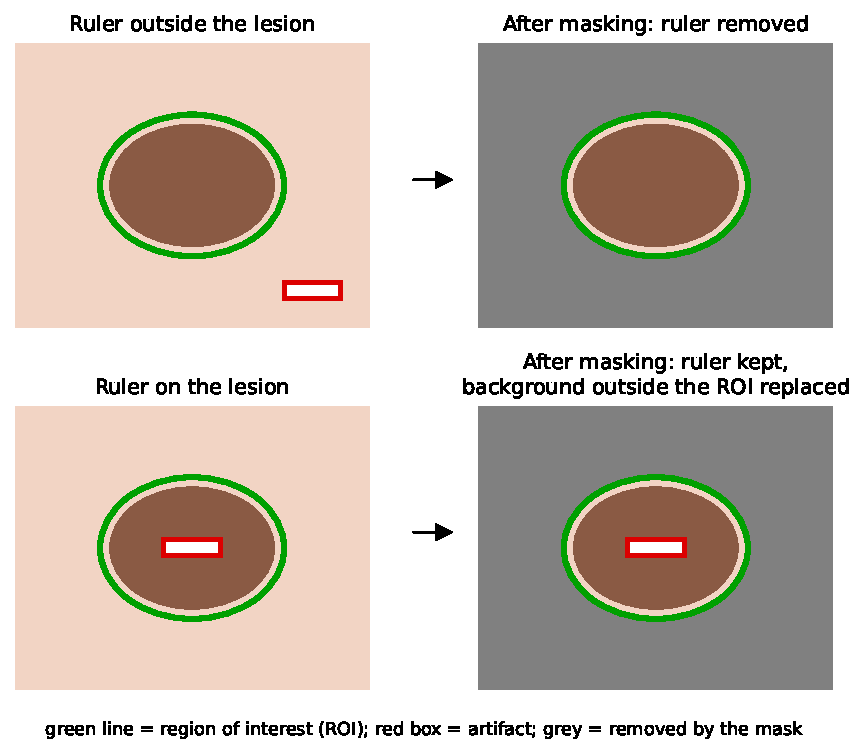
\includegraphics[width=0.42\linewidth]{figures/masking_idea.pdf}
\caption{The idea. Top: an artifact outside the lesion is deleted by the mask. Bottom: an artifact on the lesion
survives the mask, while everything that competed with it is deleted.}\label{fig:idea}\end{figure}

\textbf{Research question.} \emph{Does the benefit of ROI masking depend on where the artifact sits relative to the
ROI? If so, why, and does it hold for real artifacts and other kinds of medical images?}

\section{How we test it}
\paragraph{Two models} Every experiment compares two models that use the same frozen image encoder (a pretrained
foundation model; mainly DINOv2 ViT-B/14 at 518 px \citep{oquab2024dinov2}) and the same simple classifier on top
(logistic regression whose settings are chosen on clean validation images):
\begin{itemize}[leftmargin=1.2em,itemsep=1pt,topsep=2pt]
\item the \textbf{standard model} sees the whole image;
\item the \textbf{masked model} sees the image with everything outside the ROI replaced by the image's average
colour, in training and in testing.
\end{itemize}
The two models share the frozen encoder, the classifier type and the training recipe; only the input differs. Each
classifier is trained with 3 random seeds in the pasted-artifact experiments. In the real-artifact experiments it is
trained with 5 seeds, and for each seed on 5 grouped folds (25 fits per model). The folds are grouped by lesion for skin;
the other datasets publish no patient identifiers, so there we group near-identical images (and, for capsule images,
blocks of consecutive frames).

\paragraph{The trap} To measure how much a model relies on the artifact, we build a ``trap''
(Figure~\ref{fig:env}). In the training data the artifact appears on 90\% of the images of the target class (e.g.\ melanoma) and 10\%
of the other class, so it is a strong shortcut. We then test on three test sets:
\begin{itemize}[leftmargin=1.2em,itemsep=1pt,topsep=2pt]
\item \textbf{correlated test}: same 90/10 pattern as in training. A shortcut model looks good here.
\item \textbf{reversed test}: the pattern is flipped (10/90). A model that uses the artifact \emph{fails} here.
\item \textbf{clean test}: the artifact tells nothing about the disease (pasted-artifact experiments: no artifact;
real-artifact experiments: artifact on half of each class). This shows how well the model knows the disease itself.
\end{itemize}
\begin{figure}[!htb]\centering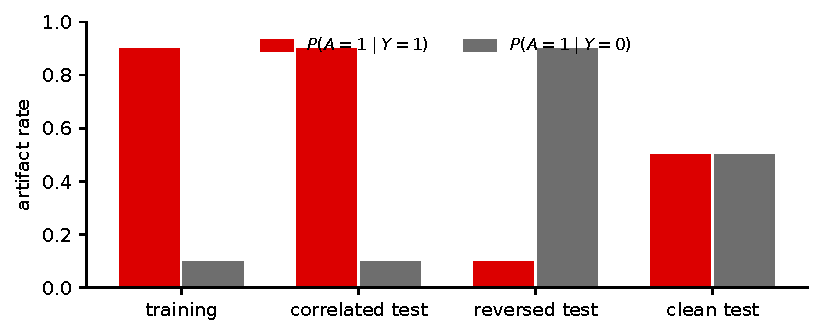
\includegraphics[width=0.38\linewidth]{figures/environments.pdf}
\caption{The trap. Bars show how often the artifact appears in the target class (red) and the other class (grey) in
training and in each test set. The clean test shown (50/50) is the one of the real-artifact experiments; in the
pasted-artifact experiments the clean test has no artifact.}\label{fig:env}\end{figure}

\paragraph{The score} We report AUROC (0.5 = guessing, 1.0 = perfect). Our main score is the AUROC on the
\emph{reversed} test. A higher reversed-test AUROC means better discrimination when the artifact--label link is
reversed. It does not directly measure reliance on the artifact: a model can rely on the artifact and still score well
if it also knows the disease well. We usually report the
\emph{difference} ``masked minus standard''. A positive number means masking helped; a negative number means it hurt.
Square brackets give the 95\% confidence interval (10,000 bootstrap replicates; see ``Honest error bars''); if it
does not include zero, the difference is significant.
The \textbf{location effect} is this difference with the artifact outside the ROI minus the same difference with the
artifact fully inside. A positive location effect means masking helps more when the artifact is outside.

\needspace{8\baselineskip}\paragraph{Measuring fairly} Two details turned out to matter.
\begin{itemize}[leftmargin=1.2em,itemsep=1pt,topsep=2pt]
\item \textbf{Near-duplicate images.} Skin-lesion datasets contain several photos of the same lesion. If one copy is in
training and another in testing, the test partly measures memory. We always split by lesion (and by image similarity),
never by single images. With random splits, 93 near-duplicate pairs crossed the split and the measured shortcut was
10--18\% too large (shortcut gap 0.284 vs 0.241 with the ruler outside, 0.465 vs 0.421 inside).
\item \textbf{Honest error bars.} We train each model several times, and the runs share test images. In the
pasted-artifact experiments, all three seeds score one fixed test set (356 images, 73 melanomas; training 1,735,
validation 346). In the real-artifact experiments, each of the 5 seeds tests every image once over its 5 folds, so the
seeds' test sets overlap heavily. A common way of computing confidence intervals treats every run as if it had its own
test set, which makes the intervals too narrow. Instead, each bootstrap replicate resamples the seeds and gives each
test image one random weight that it keeps in every seed, in both models and (for the crossover) in both traps; the
compared numbers are therefore always paired on the same images. The weights belong to single images, not to
patients or lesions, so several images of one lesion or patient are not resampled together; where these exist, our
intervals may still be somewhat too narrow. Our intervals are about 1.5 times wider than the
common method's, and a few results that looked significant with it are not.
\end{itemize}
Before each main experiment we wrote down the design and what result would count as support, and stored it in the
project repository. Results are reported whichever way they went.



\section{Step 1: moving a ruler into the lesion}\label{sec:ruler}
\paragraph{What we did} We first wanted to change \emph{only} the location of the artifact. We took 2,437 dermoscopy
images with manual lesion masks (ISIC 2018 \citep{codella2019isic}; task: melanoma or not) and pasted the same
ruler into each image at 0, 25, 50, 75 or 100\% overlap with the lesion (Figure~\ref{fig:ruler}). Only the ruler's
position changes: same images, same ruler, same labels.
\begin{figure}[!htb]\centering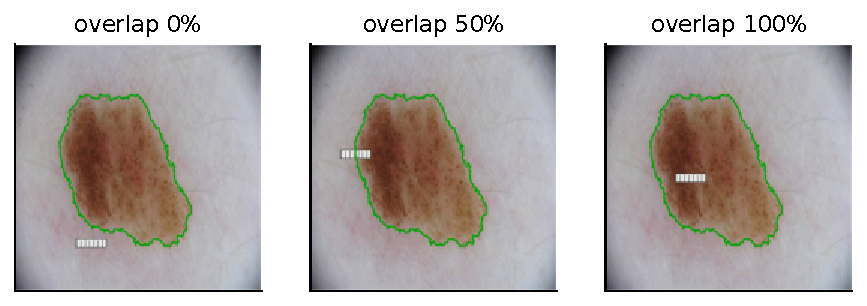
\includegraphics[width=0.52\linewidth]{figures/ruler_examples.pdf}
\caption{The same image with the ruler at 0, 50 and 100\% overlap with the lesion (green: lesion mask).}
\label{fig:ruler}\end{figure}

\paragraph{What we found} When the ruler lies outside the lesion, masking removes it and helps a lot ($+0.18$). From
50\% overlap on, masking \emph{hurts}: at full overlap the masked model is worse than the standard model ($-0.13$;
Table~\ref{tab:ruler}, Figure~\ref{fig:sweep}). The correlated test shows why: with the ruler on the lesion, the masked
model scores \emph{higher} than the standard model there (0.961 vs 0.937) but lower on the reversed test (0.386 vs
0.515). It has become \emph{more} dependent on the ruler.
\begin{table}[!htb]\centering\small
\caption{Ruler experiment (DINOv2, AUROC, mean of 3 seeds). The last row is the effect of masking on the reversed
test.}\label{tab:ruler}
\resizebox{\linewidth}{!}{\begin{tabular}{lccc}\toprule
 & Ruler outside (0\%) & Half on the lesion (50\%) & Fully on the lesion (100\%) \\\midrule
Standard model, reversed test & 0.665 & 0.573 & 0.515 \\
Masked model, reversed test & 0.849 & 0.476 & 0.386 \\
Standard model, correlated test & 0.906 & --- & 0.937 \\
Masked model, correlated test & 0.849 & --- & 0.961 \\\midrule
\textbf{Masked $-$ standard (reversed)} & $\mathbf{+0.184}$ [$+0.117, +0.250$] & $\mathbf{-0.097}$ [$-0.164, -0.030$] & $\mathbf{-0.129}$ [$-0.195, -0.064$] \\
\bottomrule\end{tabular}}\end{table}
\begin{figure}[!htb]\centering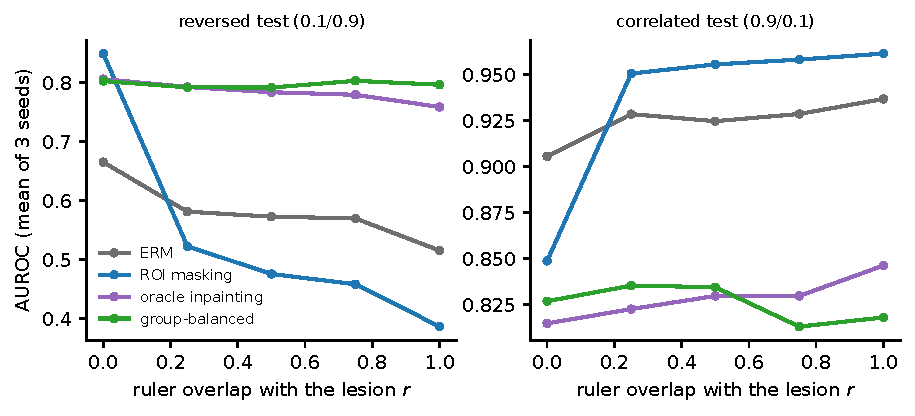
\includegraphics[width=0.58\linewidth]{figures/ruler_sweep.pdf}
\caption{AUROC on the reversed test (left) and the correlated test (right) as the ruler moves into the lesion.
Blue: masked model; grey: standard model. For comparison: purple, painting out the ruler (needs the ruler's
outline); green, balanced reweighting (needs to know which images have a ruler).}\label{fig:sweep}\end{figure}

\paragraph{Is it a fluke of one model or one ruler?} No. We repeated the experiment with a lower image resolution (224 px), with a
dermatology-specific encoder (DermLIP \citep{yan2025derm1m}), and with a ruler whose colour, ticks and size change from
image to image. The location effect was large and positive every time (Table~\ref{tab:rep}, first four rows).
\begin{table}[!htb]\centering\small
\caption{The ruler result repeated with other settings (masked $-$ standard, reversed test).}\label{tab:rep}
\resizebox{\linewidth}{!}{\begin{tabular}{lccc}\toprule
Setting & Ruler outside & Ruler fully inside & Location effect \\\midrule
DINOv2, 518-px images (main result) & $+0.184$ & $-0.129$ & $+0.313$ [$+0.258, +0.370$] \\
DINOv2, 224-px images & $+0.361$ & $-0.095$ & $+0.456$ [$+0.390, +0.525$] \\
DermLIP (dermatology encoder) & $+0.161$ & $-0.263$ & $+0.424$ [$+0.335, +0.517$] \\
DINOv2, randomised ruler & $+0.146$ & $-0.155$ & $+0.302$ [$+0.248, +0.357$] \\\midrule
\multicolumn{4}{l}{\emph{Two ruler sizes on the same 1,314 images:}} \\
DINOv2, ruler 13\% of the image width & $+0.160$ & $-0.102$ & $+0.262$ [$+0.200, +0.325$] \\
DINOv2, ruler 39\% of the image width & $+0.170$ & $-0.054$ & $+0.224$ [$+0.161, +0.285$] \\
\textbf{Average of the two sizes} & $\mathbf{+0.165}$ & $\mathbf{-0.078}$ & $\mathbf{+0.243}$ [$+0.182, +0.304$] \\
\bottomrule\end{tabular}}\end{table}

\paragraph{Different ruler sizes} Real rulers come in different sizes. We therefore ran two sizes, 13\% and 39\% of
the image width (the wider one thin, with millimetre ticks, like a real scale bar), on the 1,314 images whose lesions
can hold both fully inside (last three rows of Table~\ref{tab:rep}). The design was written down before the run; the
average was added afterwards. Both sizes show a clear location effect ($+0.262$ and $+0.224$). Averaged over the two,
masking helps by $+0.165$ with the ruler outside and hurts by $-0.078$ [$-0.149, -0.010$] with it fully on the lesion.
For the 39\% ruler alone, that harm is not significant ($-0.054$; the interval includes zero). With both sizes, the
masked model again reacts to the ruler on the lesion about twice as strongly as the standard model (check~3 below).

\section{Step 2: why does masking fail?}
Step~1 showed \emph{that} masking fails when the ruler is inside. There were three possible reasons:
(a) masking simply hides useful parts of the image; (b) the background holds disease information that masking throws
away; (c) the ruler inside the lesion survives, and because masking deletes everything that competed with it, the model
relies on it more. We designed one check for each (Table~\ref{tab:why}).

\begin{table}[!htb]\centering\small
\caption{Four checks of why masking fails (ruler experiment, DINOv2).}\label{tab:why}
\resizebox{\linewidth}{!}{\begin{tabular}{P{3.3cm}P{4.6cm}P{4.4cm}P{3.6cm}}\toprule
Check & What we changed & Result & What it means \\\midrule
1. Useless ruler & Ruler at the same places, but \emph{unrelated} to the diagnosis & No statistically clear harm at any position (all intervals include 0; e.g.\ $+0.039$ at 100\%) & Supports dependence on the ruler as a shortcut; does not exclude an effect of hiding image parts (speaks against a as the main cause) \\
2. Bigger mask & Grow the mask around the lesion: more skin comes back, and more of a half-covered ruler stays visible (50\% $\to$ 95\% of the ruler) & Harm gets \emph{worse}: $-0.097 \to -0.153$. When the ruler is already fully visible, the point estimates were similar ($-0.129$ vs $-0.138$) & At 50\% skin and ruler come back together; at 100\% only skin comes back and the estimates were similar. Speaks against b as the main cause \\
3. Same-image test & Add or remove the ruler on the \emph{same} test image and measure how much the predicted probability (0 to 1) changes & The masked model's prediction changes about twice as much as the standard model's (0.49 vs 0.24; with the 39\% ruler 0.43 vs 0.21) & The masked model leans more on the ruler (supports c) \\
4. Lesion size & Split test images into small, medium and large lesions & Harm with the ruler inside: small $-0.36$, medium $-0.16$, large $+0.06$ (not significant) & Harm is largest where the ruler is big compared to the lesion \\
\bottomrule\end{tabular}}\end{table}

\keybox{\textbf{Explanation.} Masking deletes everything outside the ROI. If the artifact is outside, the shortcut is
gone. If the artifact is inside, it survives, and the other image information that used to compete with it is gone, so
the artifact becomes a bigger part of what the model can use. The model relies on it more, and fails when the
artifact is missing or misleading.}

\section{Step 3: is it only skin images?}
\paragraph{What we did} We repeated the moving-artifact experiment in four other kinds of medical images, each with its
own typical artifact and its own ROI (Figure~\ref{fig:sweepex}): a sonographer's caliper on \textbf{thyroid
ultrasound} (TN3K, malignant or benign nodule \citep{gong2021tn3k}) and on \textbf{ovarian ultrasound} (MMOTU
\citep{zhao2022mmotu}; our grouping of its diagnoses, normal ovaries excluded; tumour with a solid part: teratoma, theca cell tumour, mucinous cystadenoma, high-grade serous
carcinoma; cystic: chocolate cyst, serous cystadenoma, simple cyst); a debris blob on \textbf{capsule endoscopy} (SEE-AI, erosion or
polyp-like lesion \citep{seeai2023}); and a tube on \textbf{chest X-rays} (NIH ChestX-ray14, pneumothorax
\citep{wang2017chestxray8}; ROI = the lungs). We used only images without a real artifact, so the pasted one was the only
one. We also tested a second encoder where possible (MedSigLIP, a medical image model; RAD-DINO, a chest X-ray model
\citep{perezgarcia2025raddino}).
\begin{figure}[!htb]\centering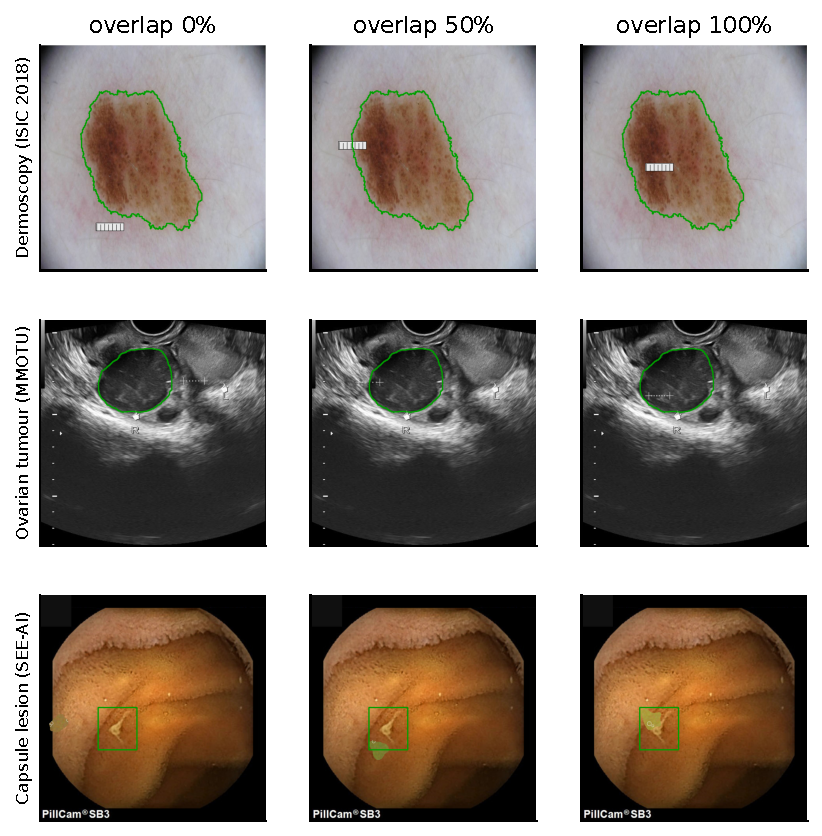
\includegraphics[width=0.44\linewidth]{figures/sweep_examples.pdf}
\caption{The pasted artifact at 0, 50 and 100\% overlap in three modalities (green: ROI; for capsule images the ROI is
the expert's box around the lesion).}\label{fig:sweepex}\end{figure}

\paragraph{What we found} Counting the first four rows of Table~\ref{tab:rep} and the seven rows of
Table~\ref{tab:other}, the location effect was positive in 10 of 11 experiments (Figure~\ref{fig:all}). Masking helped
clearly when the artifact was outside and lost most or all of its benefit when it was inside. Whether masking actually
\emph{hurt} at full overlap depended on the setting: it hurt significantly in 7 of the 11. In thyroid ultrasound, for
example, the benefit fell from $+0.40$ to about zero.
\begin{table}[!htb]\centering\small
\caption{Moving-artifact experiments in other modalities (masked $-$ standard, reversed test).}\label{tab:other}
\resizebox{\linewidth}{!}{\begin{tabular}{llccc}\toprule
Modality and artifact & Encoder & Artifact outside & Artifact fully inside & Location effect \\\midrule
Thyroid ultrasound, caliper & DINOv2 & $+0.402$ & $-0.030$ & $+0.433$ [$+0.362, +0.507$] \\
 & MedSigLIP & $+0.514$ & $+0.044$ & $+0.470$ [$+0.388, +0.556$] \\
Ovarian ultrasound, caliper & DINOv2 & $+0.041$ & $-0.197$ & $+0.238$ [$+0.144, +0.340$] \\
Capsule endoscopy, debris & DINOv2 & $+0.116$ & $-0.112$ & $+0.228$ [$+0.144, +0.324$] \\
 & MedSigLIP & $+0.374$ & $+0.216$ & $+0.158$ [$+0.012, +0.314$] \\
Chest X-ray, tube & DINOv2 & $+0.254$ & $-0.083$ & $+0.337$ [$+0.312, +0.364$] \\
 & RAD-DINO & $-0.002$ & $+0.111$ & $-0.113$ [$-0.129, -0.097$] \\
\bottomrule\end{tabular}}\end{table}
\begin{figure}[!htb]\centering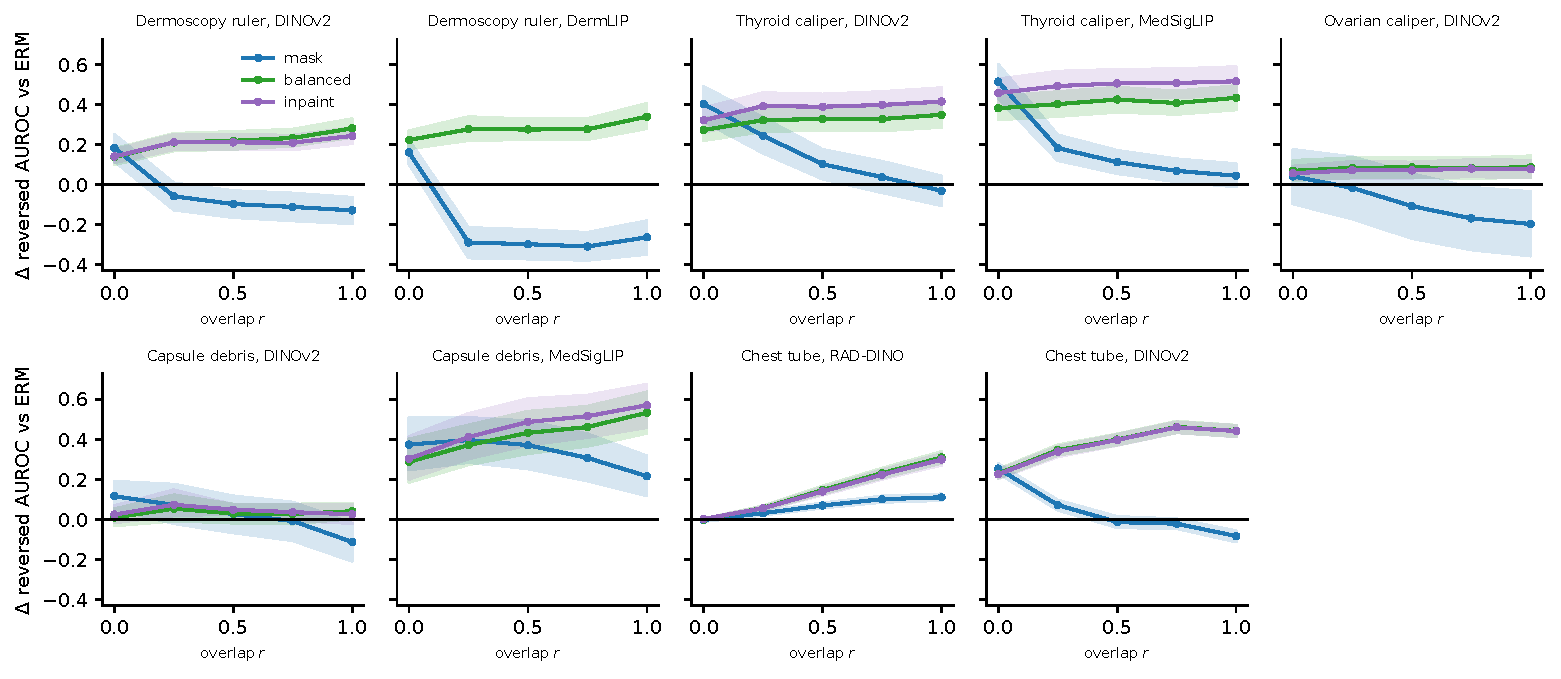
\includegraphics[width=0.64\linewidth]{figures/all_sweeps.pdf}
\caption{Effect on the reversed test (vs the standard model) as the artifact moves into the ROI, in nine of the eleven
moving-artifact experiments (the 224-px and randomised-ruler runs are in Table~\ref{tab:rep} only). Blue: masking; purple: painting out the artifact; green: balanced reweighting. The blue
line falls in every panel except the RAD-DINO chest tube.}\label{fig:all}\end{figure}

\paragraph{The one exception} With the chest X-ray encoder RAD-DINO, the standard model ignored a tube outside the
lungs (reversed AUROC 0.913, the same as on the clean test, 0.915), so masking gained nothing there, while it helped
with the tube inside the lungs ($+0.111$). This is a real exception; the likely reason is that this encoder does not use
a tube outside the lungs. With DINOv2, which did use it, the usual pattern appeared.

\section{Step 4: real artifacts}
Pasted artifacts let us control location exactly, but they are not the artifacts clinicians produce. So we next
asked whether the same thing happens with \emph{real, unedited} artifacts.

\paragraph{The design} A real artifact cannot be moved, so we compare two groups of images: those whose artifact lies
mostly inside the ROI (\textbf{Trap A}) and those whose artifact lies outside it (\textbf{Trap B}). Both traps share the
\emph{same} artifact-free images (Figure~\ref{fig:traps}). The two groups of artifact images can still differ in other
ways (lesion size, diagnosis mix, hospital, the artifact's appearance); we matched the hospital mix where there were
several hospitals, but the Trap A versus Trap B comparison remains an association with location, not a controlled
move of the artifact. Each trap gets the 90/10 training set and the three test sets of Figure~\ref{fig:env}. The
\textbf{crossover} is the benefit of masking in Trap~B minus its benefit in Trap~A; a positive crossover means masking
helps more when the artifact is outside. (We first tried comparing in-ROI with out-of-ROI images directly, without an
artifact-free group. That design cannot work: masking deletes exactly the out-of-ROI artifacts that define one side of
the comparison, so it shows ``harm'' whatever the truth.)
\begin{figure}[!htb]\centering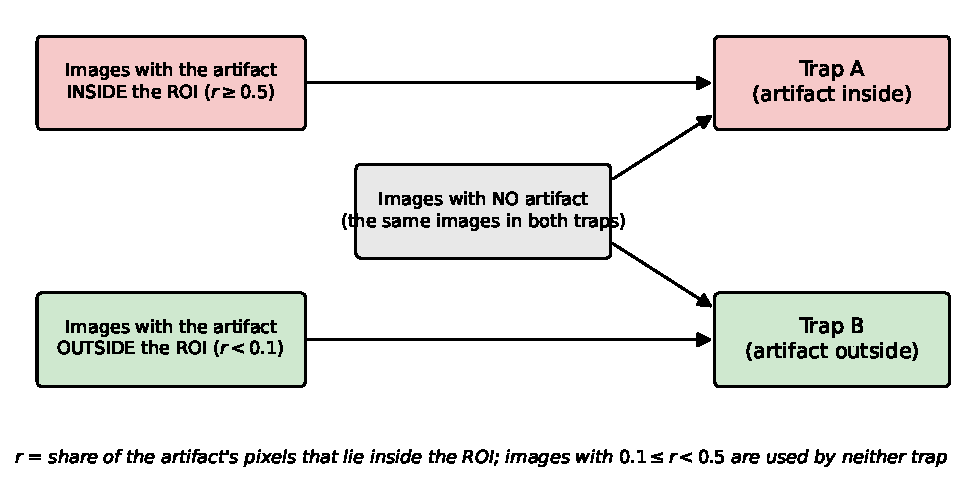
\includegraphics[width=0.55\linewidth]{figures/two_traps.pdf}
\caption{Two traps built from real images. Both share one group of artifact-free images.}\label{fig:traps}\end{figure}

\paragraph{Cohorts} Table~\ref{tab:cohorts}. Artifacts were located automatically: for skin images, published masks
that mark hair and rulers together \citep{wegley2026artifacts}, so this artifact is called ``hair/ruler''; a
rule-based caliper detector for ultrasound; and a small detector trained on expert debris masks for capsule images. We
checked them by eye: the caliper detector was right on 38 of 40 checked images. Errors in detecting the artifact or in
deciding inside versus outside may bias the crossover in either direction; measuring that needs a check of the masks
per trap and class, which we have not done yet.
\begin{figure}[!htb]\centering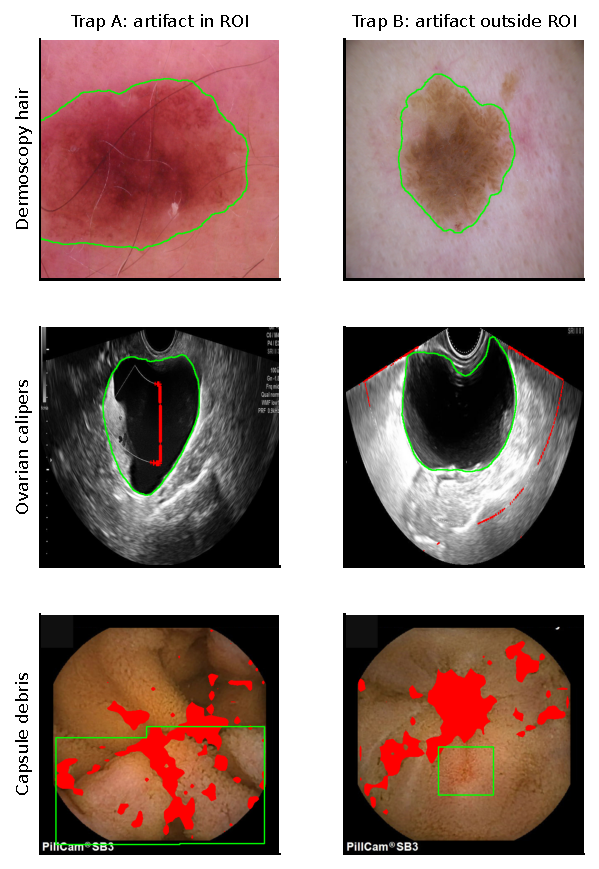
\includegraphics[width=0.34\linewidth]{figures/real_examples.pdf}
\caption{Real artifacts inside (Trap A) and outside (Trap B) the ROI. Green: ROI; red: detected artifact. (``Dermoscopy hair'' = hair/ruler masks. Thyroid images are not shown because the data licence is unclear; the
skin masks are not drawn for licence reasons.)}
\label{fig:real}\end{figure}
\begin{table}[!htb]\centering\small
\caption{The four real-artifact cohorts (number of images, target class / other class). The real-artifact
experiments use five grouped folds, so there is no fixed test split.}\label{tab:cohorts}
\resizebox{\linewidth}{!}{\begin{tabular}{P{3.6cm}P{2.6cm}P{2.6cm}ccc}\toprule
Cohort & Task & Artifact & No artifact & Trap A (inside) & Trap B (outside) \\\midrule
Skin lesions, ISIC 2019 (3 hospitals) & melanoma vs other & hair/ruler & 157 / 706 & 942 / 2,655 & 969 / 4,412 \\
Thyroid ultrasound, TN3K & malignant vs benign & calipers & 749 / 1,052 & 292 / 858 & 99 / 227 \\
Ovarian ultrasound, MMOTU & solid part vs cystic & calipers & 178 / 170 & 276 / 341 & 103 / 91 \\
Capsule endoscopy, SEE-AI & erosion vs polyp-like & debris, bubbles & 343 / 164 & 412 / 404 & 1,009 / 231 \\
\bottomrule\end{tabular}}\end{table}

\paragraph{What we found} The crossover was positive in all four cohorts with DINOv2 (Table~\ref{tab:real}). These four
tests were planned in advance; in each of them, none of the 10,000 bootstrap replicates fell at or below zero. With the
conservative two-sided formula $p = 2(k+1)/(B+1)$, where $k = 0$ replicates crossed zero and $B = 10{,}000$, this gives
$p \approx 0.0002$, and $p \approx 0.0008$ after Holm correction for four tests. It also held with MedSigLIP and with a convolutional network (ConvNeXt), so it is not specific to
one type of model; it did not hold with DermLIP (Figure~\ref{fig:forest}, Section~\ref{sec:other}).
\begin{table}[!htb]\centering\small
\caption{Real artifacts: effect of masking on the reversed test (masked $-$ standard) in each trap, and the crossover.}
\label{tab:real}
\resizebox{\linewidth}{!}{\begin{tabular}{llccc}\toprule
Cohort & Encoder & Trap A (inside) & Trap B (outside) & Crossover (B $-$ A) \\\midrule
Skin, hair/ruler & DINOv2 & $-0.049$ & $+0.098$ & $+0.147$ [$+0.111, +0.185$] \\
Thyroid, calipers & DINOv2 & $+0.109$ & $+0.348$ & $+0.239$ [$+0.196, +0.280$] \\
Ovary, calipers & DINOv2 & $+0.132$ & $+0.302$ & $+0.170$ [$+0.087, +0.252$] \\
Capsule, debris & DINOv2 & $+0.084$ & $+0.461$ & $+0.377$ [$+0.327, +0.426$] \\\midrule
Thyroid, calipers & MedSigLIP & $+0.053$ & $+0.248$ & $+0.195$ [$+0.153, +0.238$] \\
Ovary, calipers & MedSigLIP & $+0.002$ & $+0.180$ & $+0.178$ [$+0.109, +0.248$] \\
Capsule, debris & MedSigLIP & $+0.117$ & $+0.452$ & $+0.335$ [$+0.286, +0.383$] \\
Thyroid, calipers & ConvNeXt & $-0.004$ & $+0.271$ & $+0.275$ [$+0.231, +0.320$] \\
Capsule, debris & ConvNeXt & $+0.084$ & $+0.403$ & $+0.320$ [$+0.268, +0.372$] \\
Skin, hair/ruler & DermLIP & $-0.104$ & $-0.090$ & $+0.014$ [$-0.037, +0.063$] \\
\bottomrule\end{tabular}}\end{table}
\begin{figure}[!htb]\centering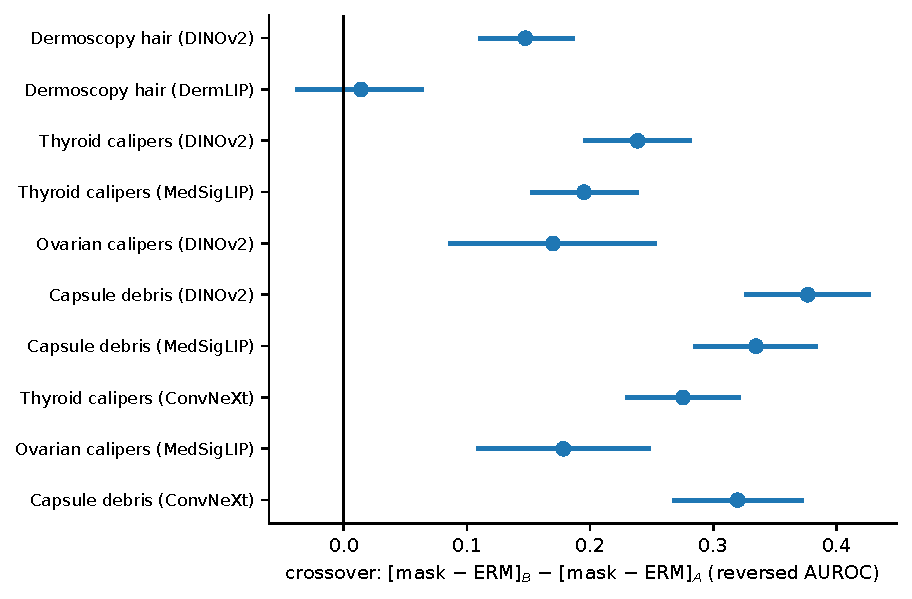
\includegraphics[width=0.46\linewidth]{figures/crossover_real.pdf}
\caption{The crossover for every cohort and encoder (dots: estimate; lines: 95\% interval). Right of zero = masking
is worth more when the artifact is outside the ROI. ``Dermoscopy hair'' = hair/ruler masks.}\label{fig:forest}\end{figure}

\paragraph{How to read it} For skin hair/ruler artifacts, masking \emph{hurt} when they lay on the lesion. For calipers and debris,
masking still helped in Trap~A, because it removes other on-screen marks and clutter, but much less than in Trap~B, and
a large part of the shortcut stayed. In thyroid Trap~A, the masked model scored 0.908 on the correlated test but only
0.398 on the reversed one; in Trap~B masking closed this gap (0.785 vs 0.752). The general rule is: \emph{masking helps
much less when the artifact is inside the ROI}. Whether it actually hurts depends on how much useful image information
masking also removes.

\section{Other things we learned}\label{sec:other}
\begin{itemize}[leftmargin=1.2em,itemsep=2pt]
\item \textbf{Methods that know which images carry the artifact help in both traps.} Reweighting the training images
so that the artifact no longer predicts the label, or retraining the last layer on a balanced subset (DFR
\citep{kirichenko2023dfr}), helped in both traps of every cohort, wherever the artifact lay (Table~\ref{tab:arms}). The
catch: reweighting needs an artifact label for every training image, and DFR for every image of its balanced subset;
clinical datasets rarely have such labels. Masking needs only the ROI.
\item \textbf{Painting out the artifact can backfire.} In capsule images, painting over the detected debris
\emph{lowered} the score ($-0.17$ in Trap~A). A likely reason is that erosions contain yellow-white material that
looks like debris, so painting it out also removes disease evidence.
\item \textbf{The hair/ruler shortcut is not only in the marked pixels.} Painting out the marked pixels closed less than
half of the standard model's shortcut gap (47\% in Trap~A, 44\% in Trap~B). The rest may come from incomplete masks,
from other artifacts, or from features that go with hair, such as age, sex and body site, which differ between the
groups; these are hypotheses we have not tested.
\item \textbf{DermLIP did not follow the rule.} With this dermatology encoder, masking hurt in \emph{both} hair/ruler
traps and there was no statistically clear crossover ($+0.014$ [$-0.037, +0.063$]). A likely reason is that it needs the skin around the lesion: masking lowered its clean-test
AUROC as well.
\item \textbf{Chest X-rays are a boundary case.} Real chest drains lie inside the lungs and are an extreme shortcut
(standard model, RAD-DINO: reversed AUROC 0.19 against 0.89 on the clean test). Lung masking barely helped (0.23),
while DFR reached 0.67. With real devices (catheters in the lungs vs breathing tubes outside them), RAD-DINO showed no
crossover and MedSigLIP a positive one in all four findings tested. The two device groups also differ in which other
devices are present, so we do not count chest X-rays as a confirmation.
\end{itemize}
\begin{table}[!htb]\centering\small
\caption{Masking against methods that use artifact labels (reversed test, change vs the standard model, DINOv2).}
\label{tab:arms}
\resizebox{\linewidth}{!}{\begin{tabular}{lcccccc}\toprule
 & \multicolumn{2}{c}{Skin, hair/ruler} & \multicolumn{2}{c}{Thyroid, calipers} & \multicolumn{2}{c}{Capsule, debris} \\
Method & Trap A & Trap B & Trap A & Trap B & Trap A & Trap B \\\midrule
ROI masking (needs ROI only) & $-0.049$ & $+0.098$ & $+0.109$ & $+0.348$ & $+0.084$ & $+0.461$ \\
Balanced reweighting (needs labels) & $+0.213$ & $+0.204$ & $+0.388$ & $+0.254$ & $+0.179$ & $+0.244$ \\
DFR (needs labels) & $+0.196$ & $+0.196$ & $+0.463$ & $+0.312$ & $+0.234$ & $+0.287$ \\
Painting out the artifact (needs its mask) & $+0.098$ & $+0.100$ & $+0.102$ & $+0.039$ & $-0.172$ & $-0.115$ \\
\bottomrule\end{tabular}}\end{table}

\section{Where we are}
\begin{table}[!htb]\centering\small
\caption{What the work so far shows.}\label{tab:sofar}
\resizebox{\linewidth}{!}{\begin{tabular}{P{4.4cm}P{8.4cm}P{4.2cm}}\toprule
Question & Answer & Evidence \\\midrule
Does masking depend on where the artifact sits? & Yes: it helps when the artifact is outside the ROI and loses its benefit (often turns harmful) when it is inside & Steps 1 and 3: 10 of 11 experiments; both ruler sizes \\
Why? & The artifact inside survives, its competitors are deleted, and the model relies on it more & Step 2: four checks \\
Does it hold for real artifacts? & Yes, in all four cohorts with DINOv2, and in every cohort tested with MedSigLIP (3) and ConvNeXt (2) & Step 4: four planned tests, all significant \\
Exceptions & DermLIP (likely needs the skin around the lesion); RAD-DINO (does not use a tube outside the lungs) & Steps 3 and 4 \\
\bottomrule\end{tabular}}\end{table}

\FloatBarrier\paragraph{Questions for discussion}
\begin{enumerate}[itemsep=1pt,topsep=2pt]
\item Is the reversed-test AUROC acceptable as the main score, or should a clinical measure (sensitivity at a fixed
specificity) be added from the start?
\item Should the rule be stated as ``masking is worth less inside the ROI'' (true in all real cohorts) rather than
``masking hurts inside the ROI'' (true for skin hair/ruler artifacts and in 7 of 11 moving-artifact experiments)?
\item The artifact masks were checked by eye by a non-clinician. Should a clinician check a sample?
\item How should chest X-rays be presented: as a boundary case, or left out of the main text?
\end{enumerate}

\renewcommand{\bibfont}{\footnotesize}\setlength{\bibsep}{0pt}
\bibliographystyle{plainnat}
\bibliography{../../stages/common/references}
\end{document}
